\documentclass[a4paper,12pt]{article}
\usepackage[ukrainian,english]{babel}
\usepackage{ucs}
\usepackage[utf8]{inputenc}
\usepackage[T2A]{fontenc}
\usepackage{amsmath}
\usepackage{fleqn}
\usepackage{amsfonts}
\usepackage{enumerate}
\usepackage{multicol}
\usepackage{forest}\usepackage{graphicx}
\begin{document}
ФІ-12 Бекешева Анастасія\\
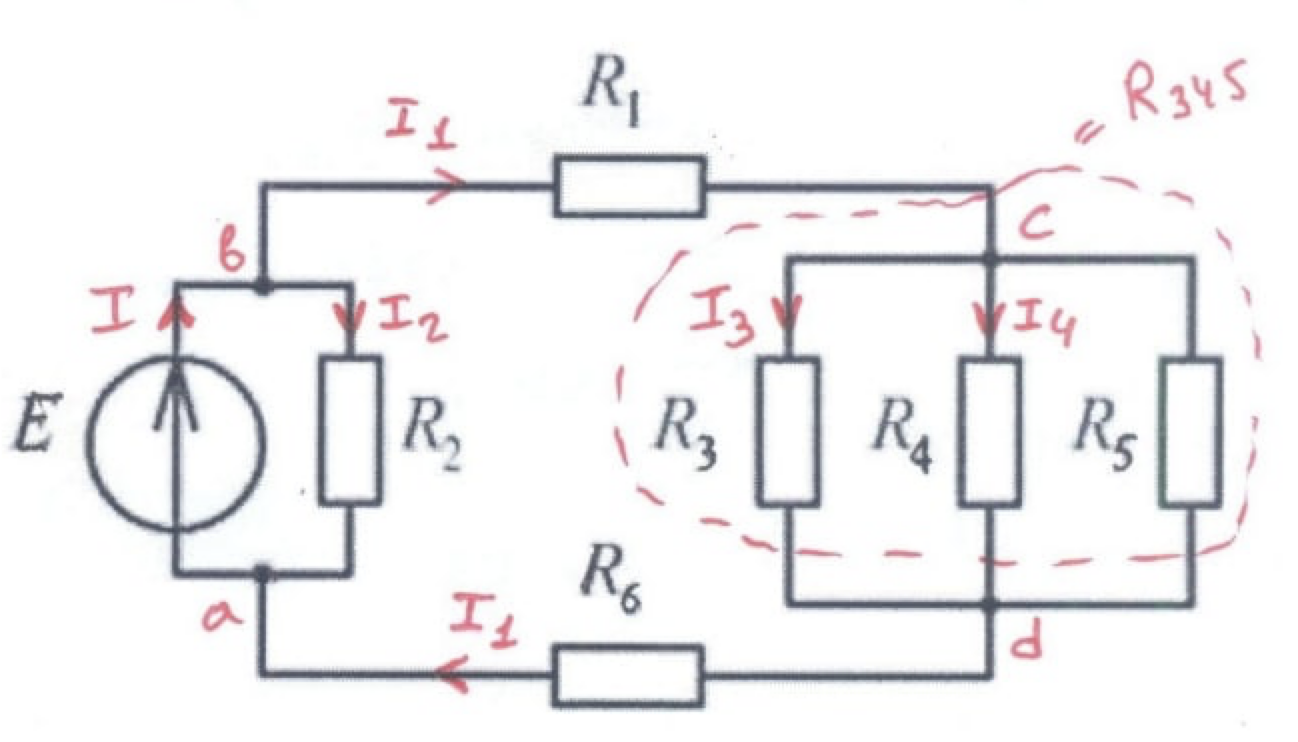
\includegraphics[width=10cm]{/Users/nastyabekesheva/Desktop/notes/physics/l5}\\
	$P_1=I_1^2R_1\Rightarrow I_1=\sqrt{\dfrac{50}4}=\dfrac{5\sqrt2}2, I_1=I_6$ - послідовне з'єднання\\$\dfrac1{R_{345}}=\dfrac1{R_3}+\dfrac1{R_4}+\dfrac1{R_5}\Rightarrow R_{345}=8,I_{345}=I_1=I_6=\dfrac{5\sqrt2}2,\>I=\dfrac UR\Rightarrow \\U_{345}=I_{345}\cdot R_{345}=20\sqrt2=U_3=U_4=U_5$ - паралельне з'эднання\\$I_3=\dfrac{5\sqrt2}{12},I_4=\dfrac{5\sqrt2}{12},I_4=\dfrac{5\sqrt2}3\\\varepsilon=U_1+U_{345}+U_6,U_1=10\sqrt2,U_6=20\sqrt2,\varepsilon=50\sqrt2=U_2\Rightarrow I_2=\dfrac{5\sqrt2}2\\P_2=250,P_3=\dfrac{50}3,P_4=\dfrac{50}3,P_5=\dfrac{200}3,P_6=100\\I_{\textrm{дж}}=I_1+I_2=5\sqrt2,P_{\textrm{дж}}=I_{\textrm{дж}}\cdot\varepsilon=500\\\dfrac1R=\dfrac1{R_2}+\dfrac1{R_1+R_{345}+R_6}=10,\displaystyle\sum P=(I_1+I_2)^2R=500$
\end{document}